\documentclass[9pt]{beamer}

\usepackage{algorithm}
\usepackage{algpseudocode}
\usepackage{amsfonts}
\usepackage{amsmath}
\usepackage{amssymb}
\usepackage{cuted}
\usepackage{hyperref}
\usepackage{lmodern}
\usepackage{mathtools}
\usepackage{multirow}
\usepackage{subcaption}
\usepackage[short]{optidef}

\usepackage{siunitx}
\DeclareSIUnit{\belmilliwatt}{Bm}
\DeclareSIUnit{\dBm}{\deci\belmilliwatt}

\usepackage{blindtext}
\newcommand\blfootnote[1]{%
\begingroup
\renewcommand\thefootnote{}\footnote{#1}%
\addtocounter{footnote}{-1}%
\endgroup
}

\usetheme{Warsaw}

\AtBeginSection
{
    \begin{frame}
        \frametitle{Table of Contents}
        \tableofcontents[currentsection]
    \end{frame}
}

\title[Waveform and Passive Beamforming Design for IRS-Aided SWIPT]{Waveform and Passive Beamforming Design for Intelligent Reflecting Surface-Aided Wireless Information and Power Transfer}
\author{Yang Zhao}
\institute{Department of Electrical and Electronic Engineering\\ Imperial College London}
\date{Early Stage Assessment, \today}

\begin{document}

\frame{\titlepage}

\begin{section}{Introduction and Review}
	\begin{subsection}{WPT}
		\begin{frame}{What is WPT?}
			\textbf{Wireless Power Transfer} (WPT) varies electromagnetic fields to deliver power.
			\vspace{1em}
			\begin{table}
				\scriptsize
				\caption{WPT Technologies}
				\begin{tabular}{|l|l|l|l|l|l|}
					\hline
					Categories                  & Technology                 & Devices           & Power                        & Frequency          & Range           \\ \hline
					\multirow{3}{*}{Near-field} & Magnetic resonant coupling & Resonators        & Up to 10 \si{\W}             & kHz -- MHz         & m               \\ \cline{2-6}
												& Inductive coupling         & Wire coils        & Up to 10 \si{\W}             & Hz -- MHz          & mm -- cm        \\ \cline{2-6}
												& Capacitive coupling        & Metal plates      & Up to 1 \si{\W}              & kHz -- MHz         & mm              \\ \hline
					\multirow{2}{*}{Far-field}  & \alert{RF waves}           & \alert{Rectennas} & \alert{\si{\uW} -- \si{\mW}} & \alert{MHz -- GHz} & \alert{m -- km} \\ \cline{2-6}
												& Light waves                & Lasers            & \si{\uW} -- \si{\mW}         & THz                & km              \\ \hline
				\end{tabular}
			\end{table}
			\vspace{1em}
			\textbf{Characteristics}:
			\begin{itemize}
				\item no wires and batteries
				\item everlasting, controllable, reliable, sustainable
			\end{itemize}
		\end{frame}

		\begin{frame}{WPT by RF waves}
			\textbf{Energy flow}: DC $\to$ \alert{RF $\to$ RF $\to$ DC}
			\begin{figure}
				\centering
				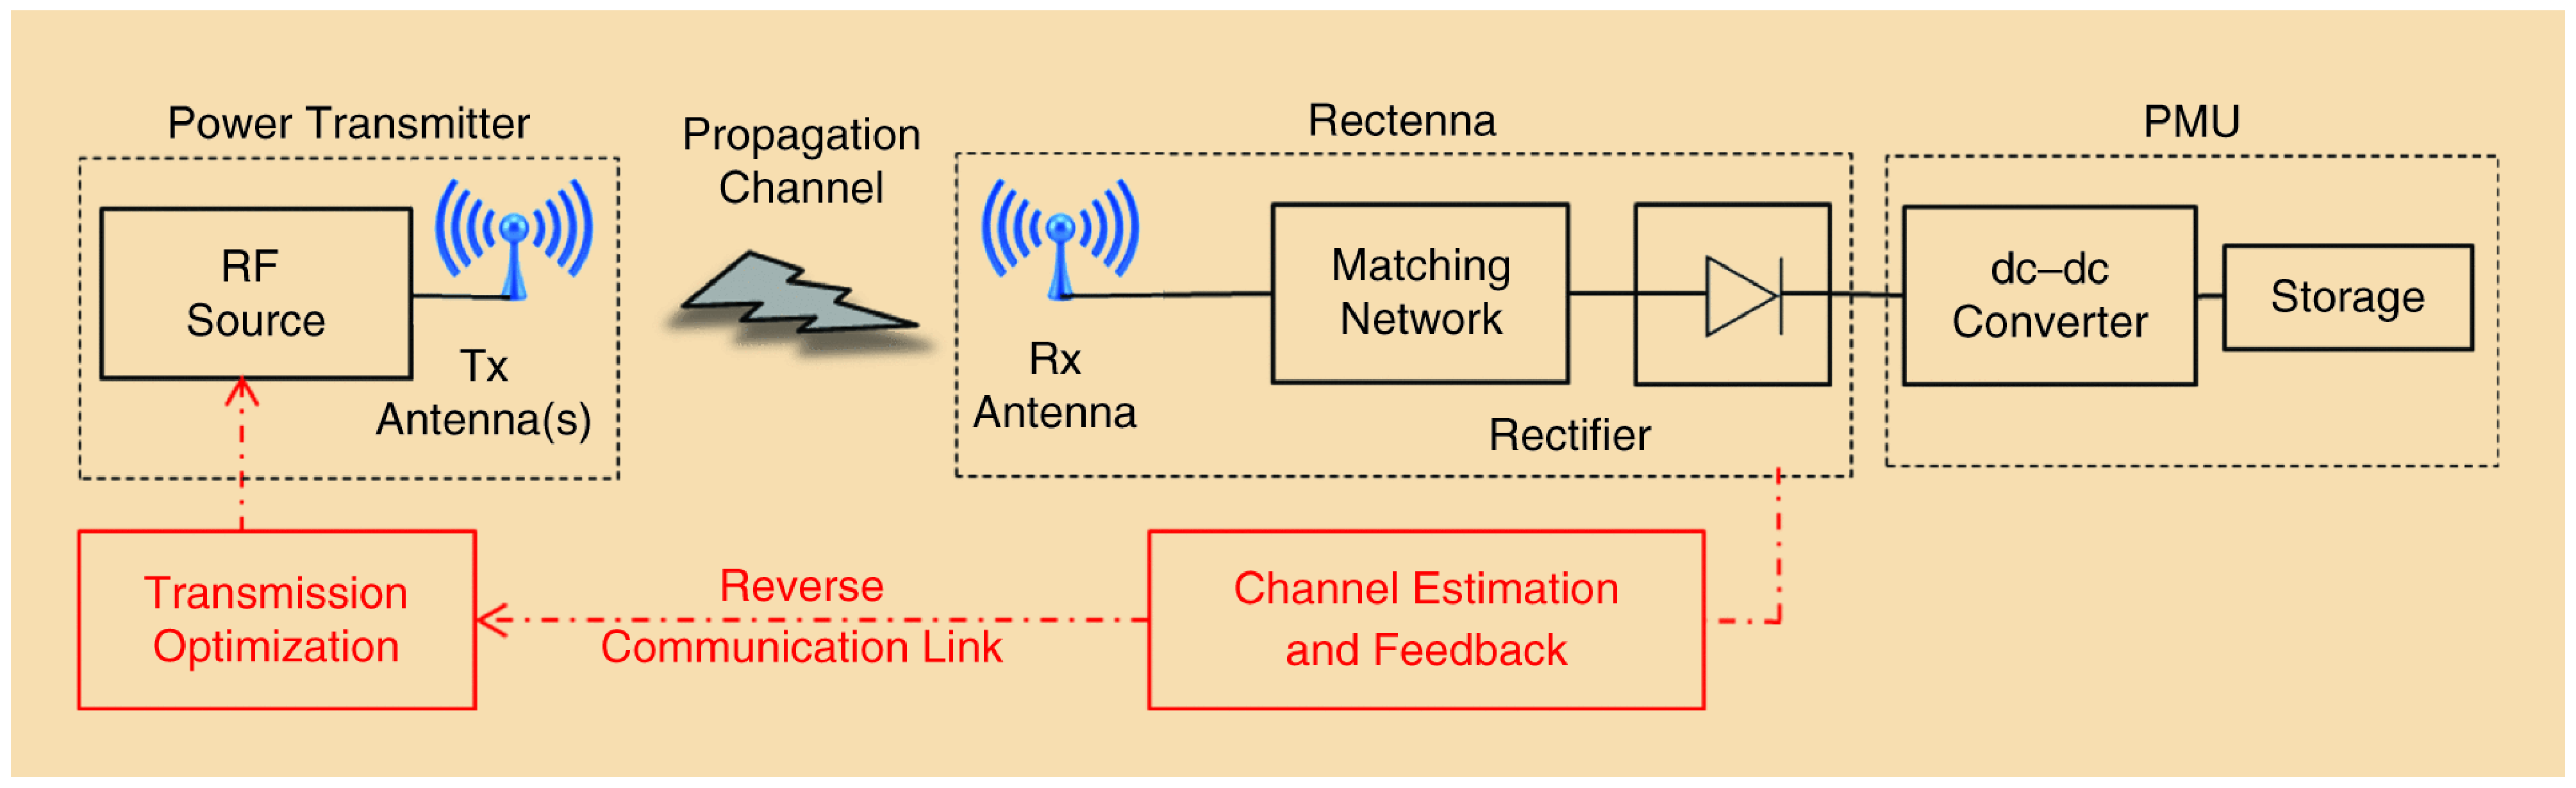
\includegraphics[width=\textwidth]{assets/wpt.eps}
			\end{figure}
			\textbf{Pros}:
			\begin{itemize}
				\item long range (up to hundreds of \si{\m}) with NLoS support
				\item compact receiver (few \si{\cm}), easy integration
				\item suitable for mobile devices
			\end{itemize}
			\textbf{Cons}:
			\begin{itemize}
				\item low power level (\si{\uW} -- \si{\mW})
				\item low energy harvesting efficiency (40\% at 100 \si{\uW}, 20\% at 10 \si{\uW})
			\end{itemize}
			\blfootnote{Figure from \cite{Clerckx2018a}}
		\end{frame}
	\end{subsection}

	\begin{subsection}{SWIPT}
		\begin{frame}{Why RF waves?}
			RF waves enables:
			\begin{itemize}
				\item Wireless communication (WIT)
				\item WPT
			\end{itemize}
			\vspace{1em}
			\textbf{Simultaneous Wireless Information and Power Transfer} (SWIPT): downlink WIT and WPT at the same time. Receivers can be either separated or \alert{co-located}.
			\vspace{1em}
			\begin{figure}
				\centering
				\begin{subfigure}{0.48\textwidth}
					\centering
					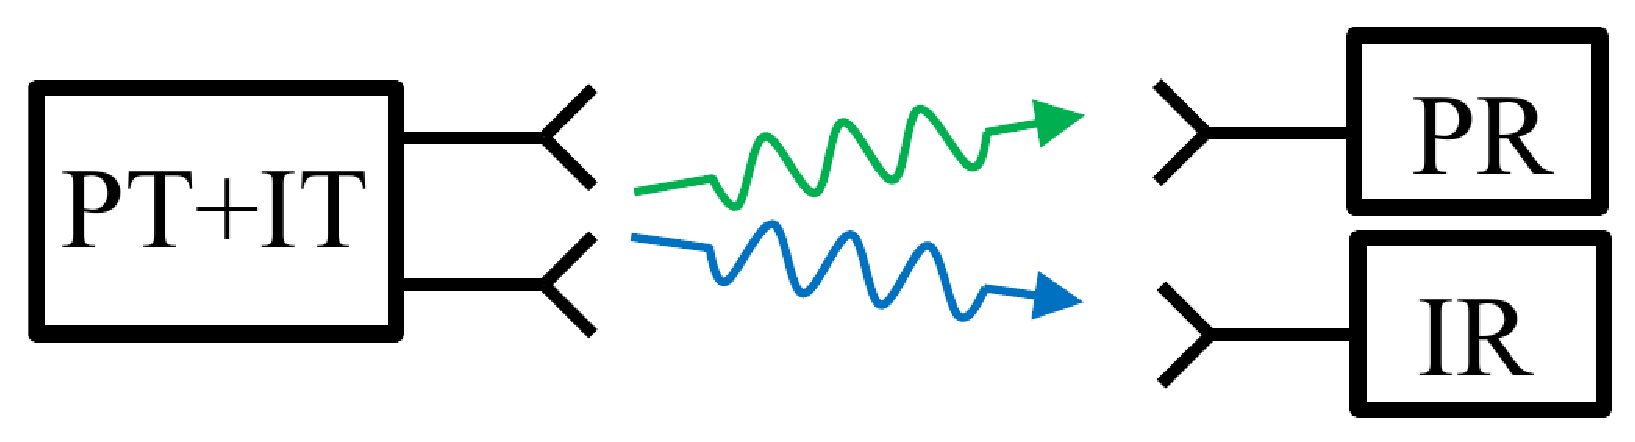
\includegraphics[width=0.8\linewidth]{assets/wipt_receiver_separated.eps}
					\caption{Separated}
				\end{subfigure}%
				\begin{subfigure}{0.48\textwidth}
					\centering
					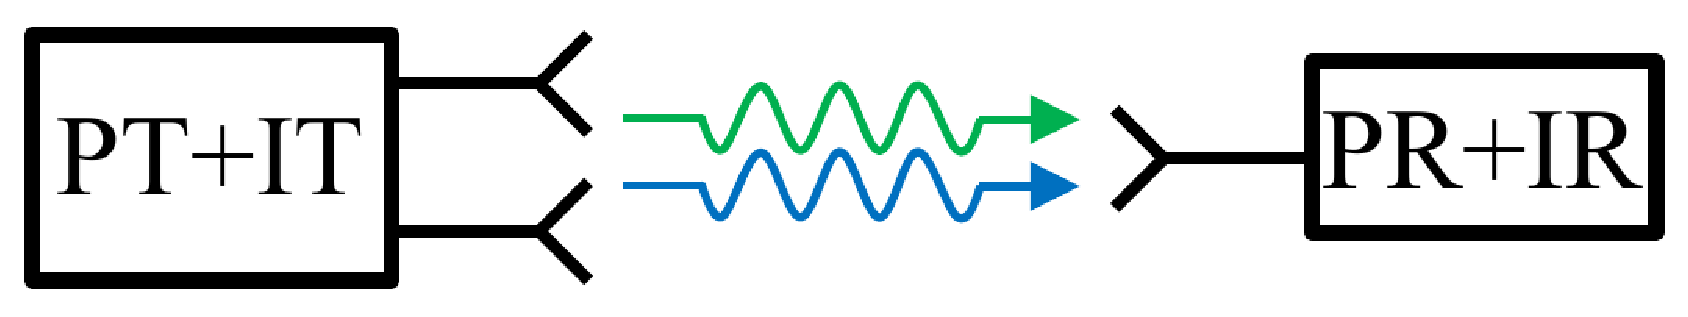
\includegraphics[width=0.8\linewidth]{assets/wipt_receiver_colocated.eps}
					\caption{Co-located}
				\end{subfigure}
				\caption{SWIPT receivers}
			\end{figure}
			\blfootnote{Figure from \cite{Clerckx2019}}
		\end{frame}

		\begin{frame}{Co-located receiver architecture}
			Two practical receiver architecture:
			\begin{itemize}
				\item \textbf{Time-Switching} (TS) switches between Information Decoding (ID) and Energy Harvesting (EH) modes on time basis.
				\item \textbf{Power-Splitting} (PS) splits the received signal into individual components for ID and EH.
			\end{itemize}
			\begin{figure}
				\centering
				\begin{subfigure}{0.48\textwidth}
					\centering
					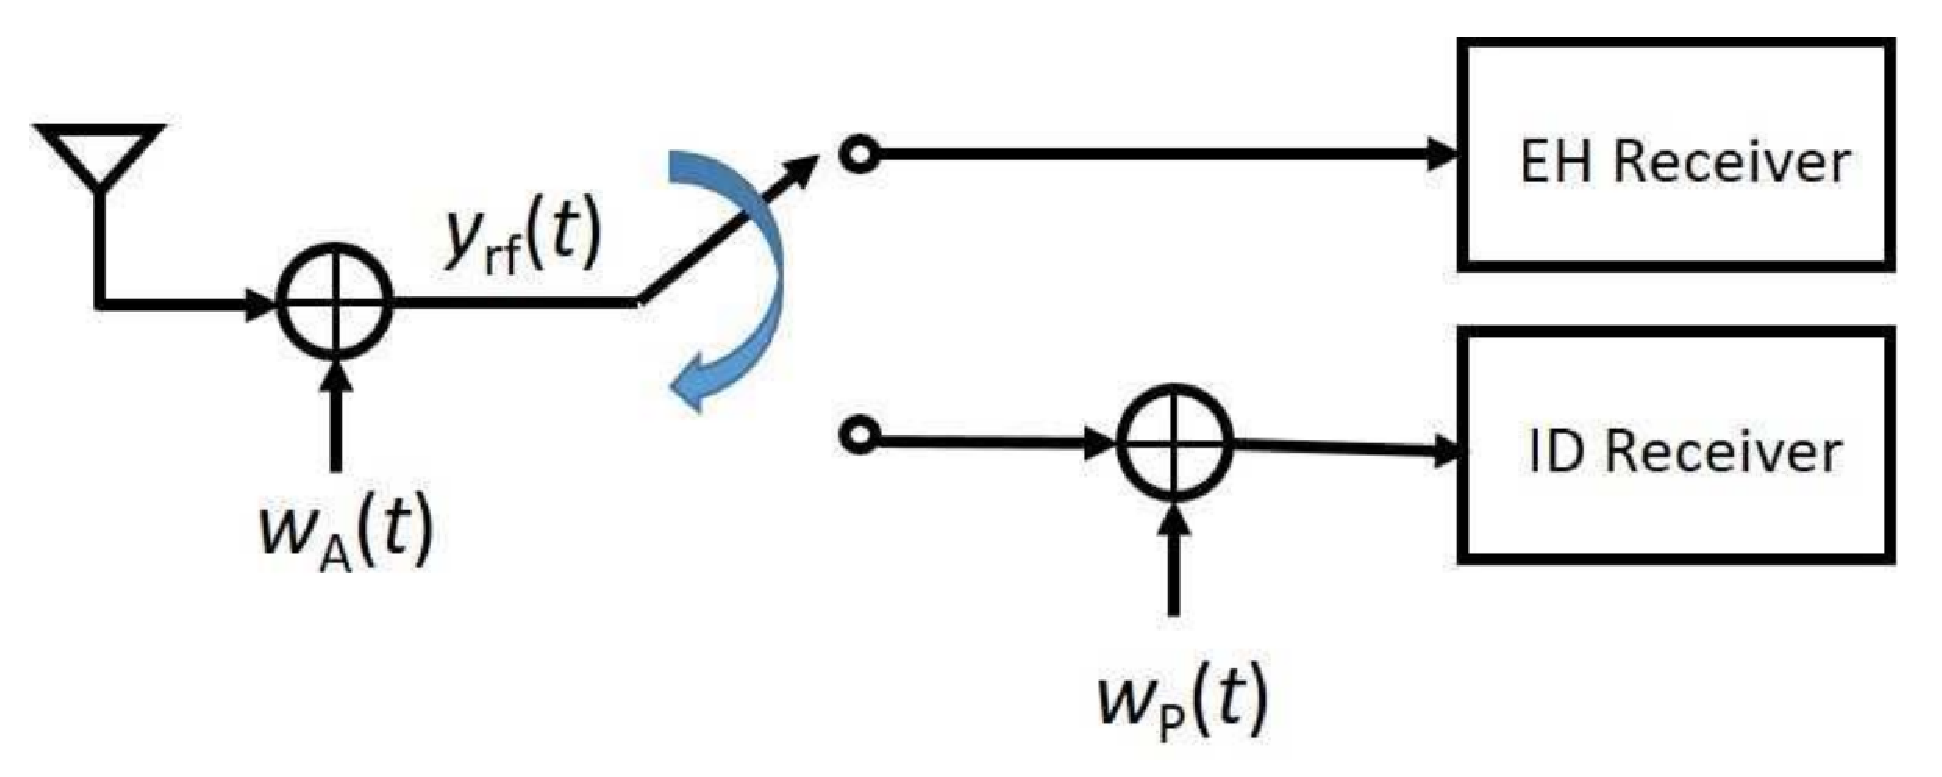
\includegraphics[width=0.8\linewidth]{assets/time_switching.eps}
					\caption{TS}
				\end{subfigure}%
				\begin{subfigure}{0.48\textwidth}
					\centering
					\includegraphics[width=0.8\linewidth]{assets/power_splitting.eps}
					\caption{PS}
				\end{subfigure}
				\caption{Co-located receiver architecture}
				\begin{block}{Design issue}
					\begin{itemize}
						\item TS can be achieved by a time sharing between WIT and WPT. Waveform is optimized individually for both cases.
						\item In PS, the splitting ratio $\rho$ is coupled with the waveform design.
					\end{itemize}
				\end{block}
			\end{figure}
			\blfootnote{Figure from \cite{Clerckx2019}}
		\end{frame}

		\begin{frame}{Harvester model}
			RF-to-DC conversion requires \textbf{rectenna} (receive antenna + rectifier), whose behavior is dominated by diode I-V characteristics.
			\begin{figure}
				\centering
				\includegraphics[width=0.8\textwidth]{assets/rectenna_circuit.eps}
				\caption{Rectenna equivalent circuit and a single diode rectifier \cite{Clerckx2018a}}
			\end{figure}
			Consider small-signal model and truncate its Taylor expansion to the $n_0$-th order:
			\begin{itemize}
				\item diode linear model (${n_o} = 2$): output power is proportional to input power
				\item \alert{diode nonlinear model} (${n_o} > 2$): contribution from high-order terms
			\end{itemize}
			\blfootnote{Figure from \cite{Clerckx2019}}
		\end{frame}

		\begin{frame}{Waveform design}
			A superposed signal containing \alert{modulated information waveform} and \alert{multisine power waveform} is demonstrated to bring a two-fold benefit:
			\begin{itemize}
				\item \textbf{rate}: multisine is deterministic with no interference on information waveform (by waveform cancellation or translated codebook)
				\item \textbf{energy}: multisine brings high PAPR and triggers the diode nonlinear model more often (reduce threshold from -20 \si{\dBm} to -30 \si{\dBm})
			\end{itemize}
			\begin{figure}
				\centering
				\begin{subfigure}{.48\textwidth}
					\centering
					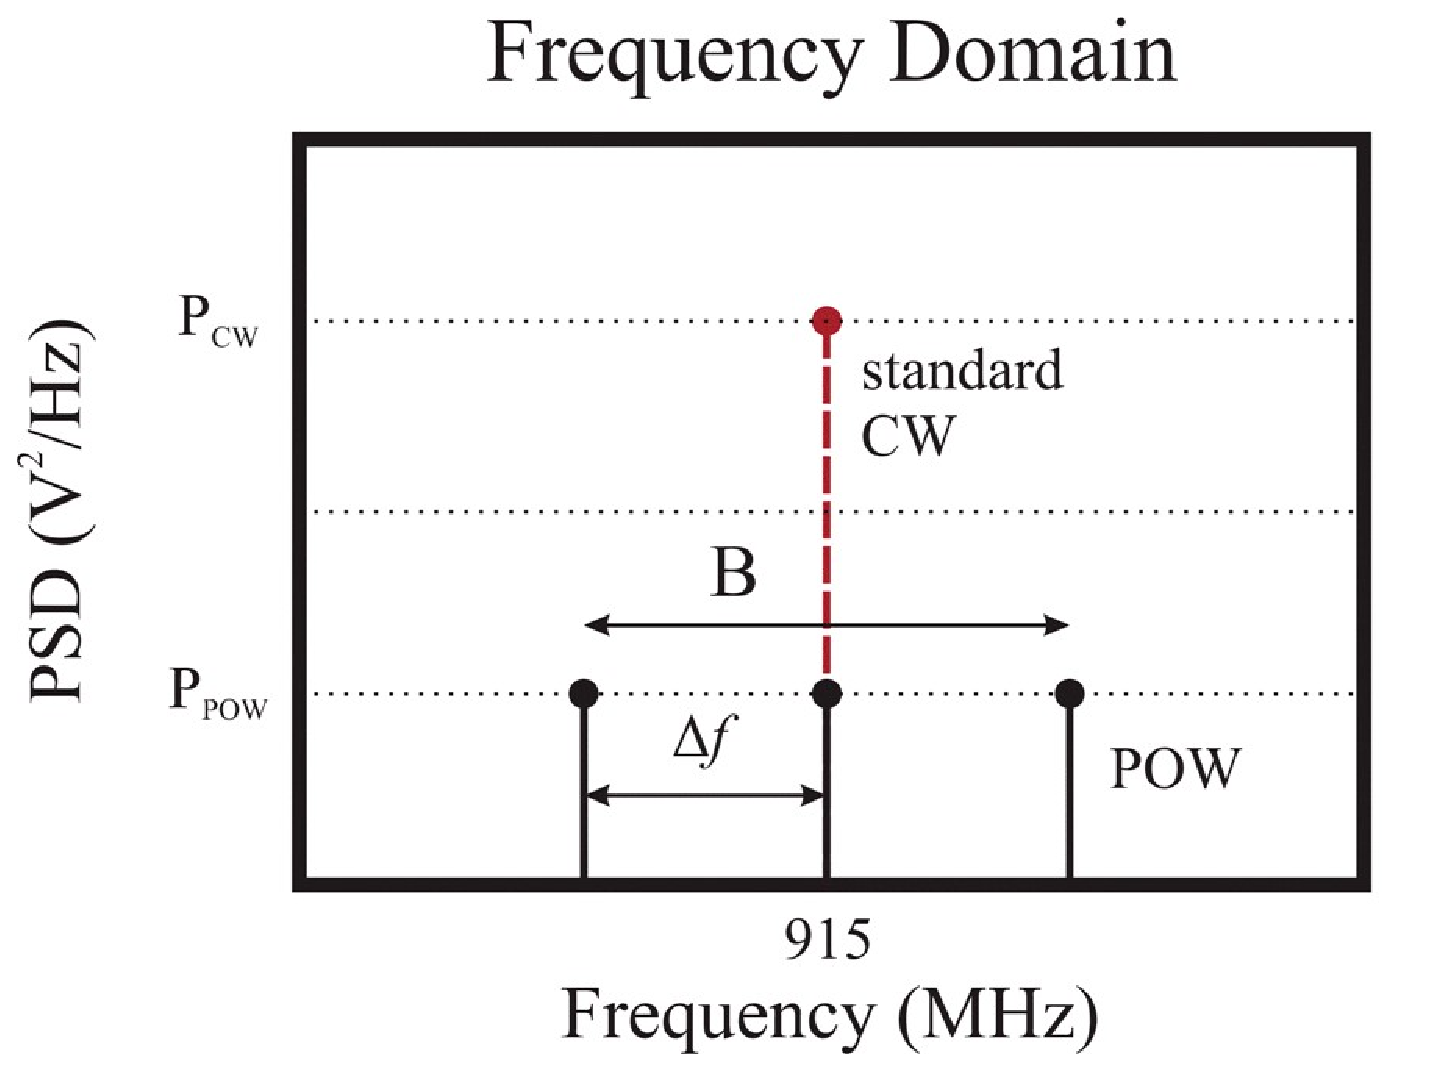
\includegraphics[width=0.8\linewidth]{assets/multisine_frequency_domain.eps}
					\caption{Frequency domain}
				\end{subfigure}
				\begin{subfigure}{.48\textwidth}
					\centering
					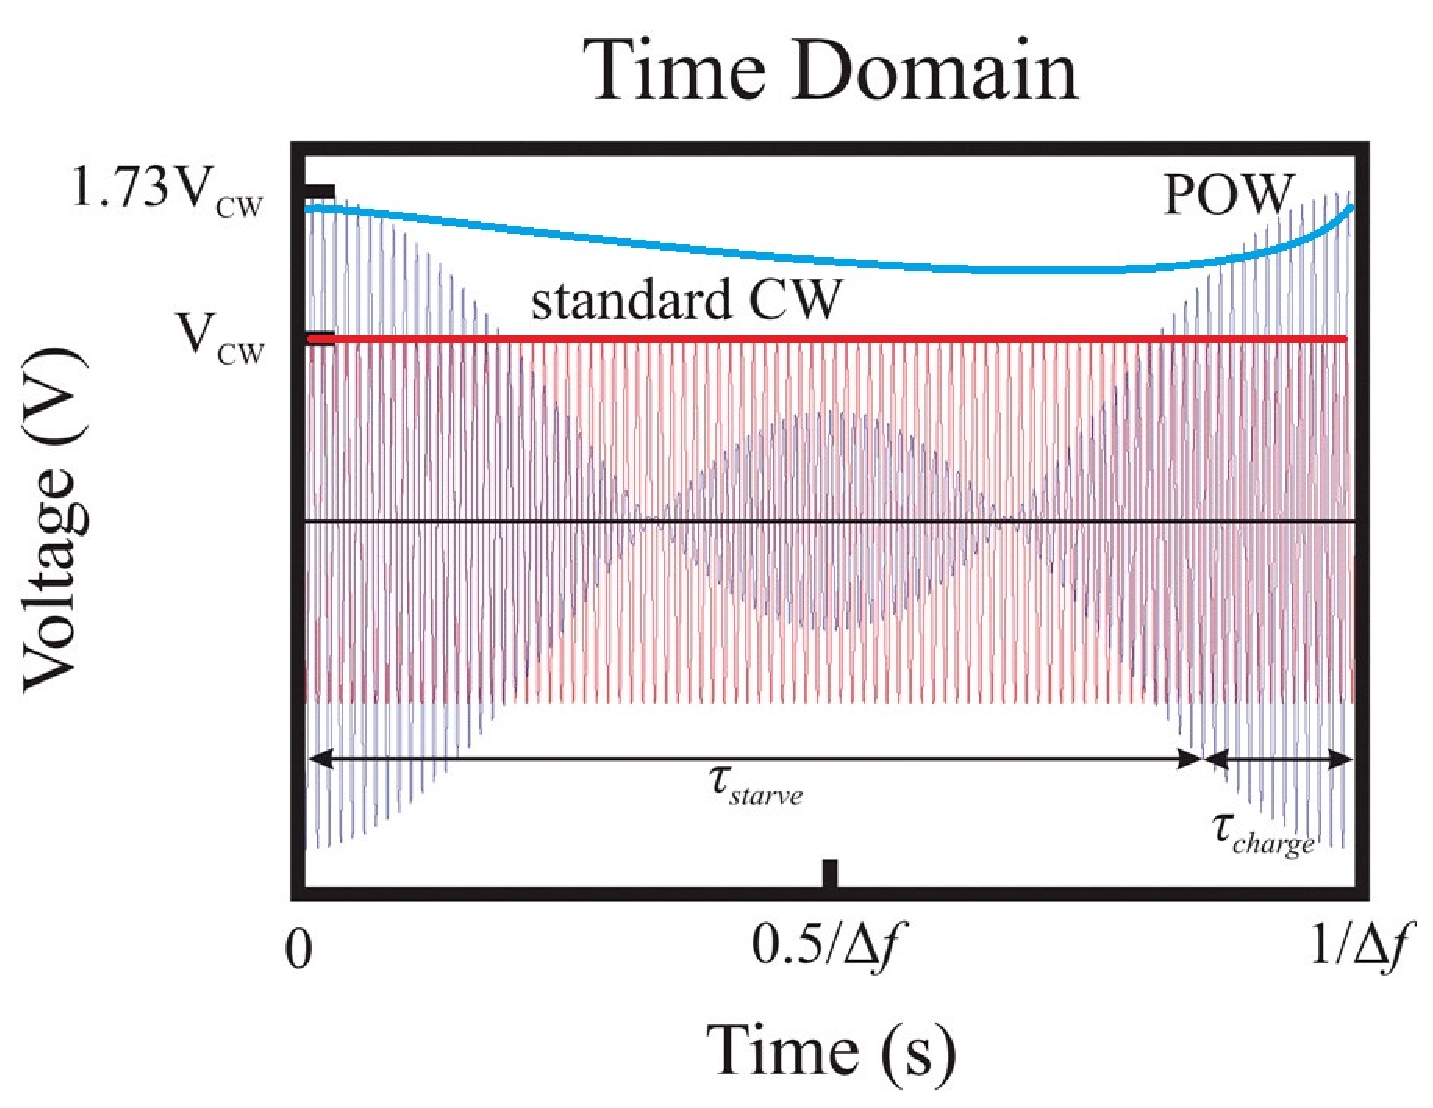
\includegraphics[width=0.8\linewidth]{assets/multisine_time_domain.eps}
					\caption{Time domain}
				\end{subfigure}
				\caption{Multisine waveform}
			\end{figure}
			\blfootnote{Figure from \cite{Trotter2009}}
		\end{frame}
	\end{subsection}

	\begin{subsection}{IRS}
		\begin{frame}{What is IRS?}
			\textbf{Intelligent Reflecting Surface} (IRS) consists of multiple individual passive reflecting elements that adjust the amplitude and phase of the incident signal.
			\begin{figure}
				\centering
				\begin{subfigure}{.48\textwidth}
					\centering
					\includegraphics[width=0.9\linewidth]{assets/irs_architecture.eps}
					\caption{IRS architecture}
				\end{subfigure}
				\begin{subfigure}{.48\textwidth}
					\centering
					\includegraphics[width=0.9\linewidth]{assets/irs_system.eps}
					\caption{Application scenario}
				\end{subfigure}
			\end{figure}
			\begin{columns}
				\begin{column}{0.5\textwidth}
					\begin{itemize}
						\item outer layer: redistribute incident signals
						\item middle layer: avoid signal energy leakage
						\item inner layer: adjust reflection amplitude and phase shift
					\end{itemize}
				\end{column}
				\begin{column}{0.5\textwidth}
					\begin{itemize}
						\item enhance primary transmission by constructive reflection
						\item null interference by destructive reflection
					\end{itemize}
				\end{column}
			\end{columns}
			\blfootnote{Figure from \cite{Wu2019,Wu2020}}
		\end{frame}

		\begin{frame}{Why IRS?}
			\textbf{Characteristics}:
			\begin{itemize}
				\item passive (different from AF relay)
				\begin{itemize}
					\item no RF chains
					\item low power consumption
					\item no additional thermal noise
					\item \alert{squared gain}: received power scales quadratically with the number of reflectors (boost receive power and array gain in equal gain transmission)
				\end{itemize}
				\item full-duplex
				\item assistant (different from backscatter node)
				\item adjustable in real-time
			\end{itemize}
			\vspace{1em}
			\textbf{Challenges}:
			\begin{itemize}
				\item channel estimation
				\begin{itemize}
					\item cannot separate incident and reflective channels
					\item large number of extra channels
				\end{itemize}
				\item practical restriction
				\begin{itemize}
					\item discrete phase shifts
					\item phase shift are coupled with reflection amplitude (by impedance equation)
				\end{itemize}
			\end{itemize}
		\end{frame}

		\begin{frame}{Why IRS-aided SWIPT?}
			\begin{itemize}
				\item both aim at improving spectral/energy efficiency
				\item enhanced channel boosts received power to benefit from harvester nonlinearity
				\item extra links increase system diversity and stability, which is essential for SWIPT
				\item SWIPT can potentially support low-power IRS
			\end{itemize}
		\end{frame}
	\end{subsection}

	\begin{subsection}{Previous research}
		\begin{frame}{Existing works}
			Separated information decoder and energy harvester:
			\begin{itemize}
				\item \cite{Wu2019b} investigated a MISO system with energy interference and proved at most one energy beam is required to maximize the WSP subject to SINR constraints.
				\item \cite{Tang2019} considered fairness issue for a MISO system and maximized the minimum output power based on perfect energy interference cancellation.
				\item \cite{Pan2019a} transformed WSR maximization of MIMO SWIPT to WMMSE problem then solved by BCD with low-complexity iterative algorithms.
				\item \cite{Wu2019c} proposed a penalty-based algorithm to minimize transmit power of MISO system subject to SINR constraints, whose inner layer updates precoders, phase shifts and auxiliary variables by BCD while the outer layer updates the penalty coefficients.
			\end{itemize}
		\end{frame}

		\begin{frame}{Outcomes and opportunities}
			\textbf{Outcomes}:
			\begin{itemize}
				\item IRS brings a significant gain to SWIPT
				\item performance vary significantly under different configuration (distances, number of reflectors, transmit power, SNR, etc.)
				\item dedicated energy beam is necessary to boost the harvested power
				\item LoS links can further increase the harvested power, since rank-deficient channels are highly correlated and a single energy stream can provide large output power for multiple harvesters
			\end{itemize}
			\vspace{1em}
			\textbf{Opportunities}:
			\begin{itemize}
				\item no works on co-located information decoder and energy harvester
				\item no works on IRS-aided OFDM SWIPT
				\item no works consider harvester nonlinearity
				\item no works investigate Rate-Energy (R-E) tradeoff
			\end{itemize}
		\end{frame}
	\end{subsection}
\end{section}

\begin{section}{System model}
	\begin{subsection}{Signal and channel}
		\begin{frame}{Signal and channel}
			SISO, $L$-reflector IRS, $K$-user, $N$-subband
			\begin{itemize}
				\item transmit signal at the AP:
				\begin{equation}
					x(t)=\Re\left\{\sum_{n=1}^N\left({w_{I,n}\tilde{x}_{I,n}(t)}+w_{P,n}\right){e^{j2{\pi}{f_n}{t}}}\right\}
				\end{equation}
				\begin{itemize}
					\item $w_{I/P,n}$ collects magnitude and phase of the information and power signal
					\item $\tilde{x}_{I,n}\sim\mathcal{CN}(0,1)$ is the information symbol
				\end{itemize}
				\item composite channel for user $k$:
				\begin{itemize}
					\item direct: AP-user ($h_{D,k,n}$)
					\item extra: AP-IRS ($\boldsymbol{h}_{I,n}$), \alert{IRS reflection ($\boldsymbol{\Theta}$)}, IRS-user ($\boldsymbol{h}_{R,k,n}^H$)
					\begin{equation}
						h_{E,k,n} = \boldsymbol{h}_{R,k,n}^H \alert{\boldsymbol{\Theta}} \boldsymbol{h}_{I,n} = \boldsymbol{v}_{k,n}^H \alert{\boldsymbol{\phi}}
					\end{equation}
					\item sum up and stack over all subbands:
					\begin{equation}
						\boldsymbol{h}_k = \boldsymbol{h}_{D,k} + \boldsymbol{V}_k^H \alert{\boldsymbol{\phi}}
					\end{equation}
				\end{itemize}
				\item received signal by user $k$
				\begin{equation}
					y_k(t)=\Re\left\{\sum_{n=1}^N{h_{{k,n}}}\left({w_{I,n}\tilde{x}_{I,n}(t)}+w_{P,n}\right){e^{j2{\pi}{f_n}{t}}}\right\}
				\end{equation}
			\end{itemize}
		\end{frame}
	\end{subsection}

	\begin{subsection}{Information decoder}
		\begin{frame}{Information decoder}
			The power component $y_{P,k}(t)$ creates no interference to the information component $y_{I,k}(t)$. Hence, the achievable rate of user $k$ is
			\begin{equation}\label{eq:R_k}
				R_k(\boldsymbol{w}_I,\boldsymbol{\phi},\rho,\boldsymbol{\alpha}_k)=\sum_{n=1}^N\alpha_{k,n}{\log_2\left(1+\frac{(1-\rho)\lvert h_{k,n}w_{I,n} \rvert^2}{\sigma_n^2}\right)}
			\end{equation}
			\begin{itemize}
				\item $\rho$ is the splitting ratio for energy harvesting
				\item $\alpha_{k,n}$ is the allocation indicator:
				\begin{equation}
					\alpha_{k,n} =
					\begin{cases}
						1, & \text{if subband } n \text{ is given to user } k \\
						0, & \text{otherwise}
					\end{cases}
				\end{equation}
				\item $\sigma_n^2$ is the variance of the noise at RF band and during RF-to-BB conversion
			\end{itemize}
		\end{frame}
	\end{subsection}

	\begin{subsection}{Energy harvester}
		\begin{frame}{Energy harvester}
			A truncated Taylor expansion of small signal model highlights the dependency of harvester output DC current on the received waveform:
			\begin{equation}
				z_k(\boldsymbol{w}_I,\boldsymbol{w}_P,\boldsymbol{\phi},\rho)=\sum_{i\,\text{even},i\ge2}^{n_0}{k_i}{\rho^{i/2}}{R_{\text{ant}}^{i/2}}{\mathcal{E}\left\{\mathcal{A}\left\{y_k(t)^i\right\}\right\}}
			\end{equation}
			Pick $n_0=4$ and we have:
			\begin{figure}
				\centering
				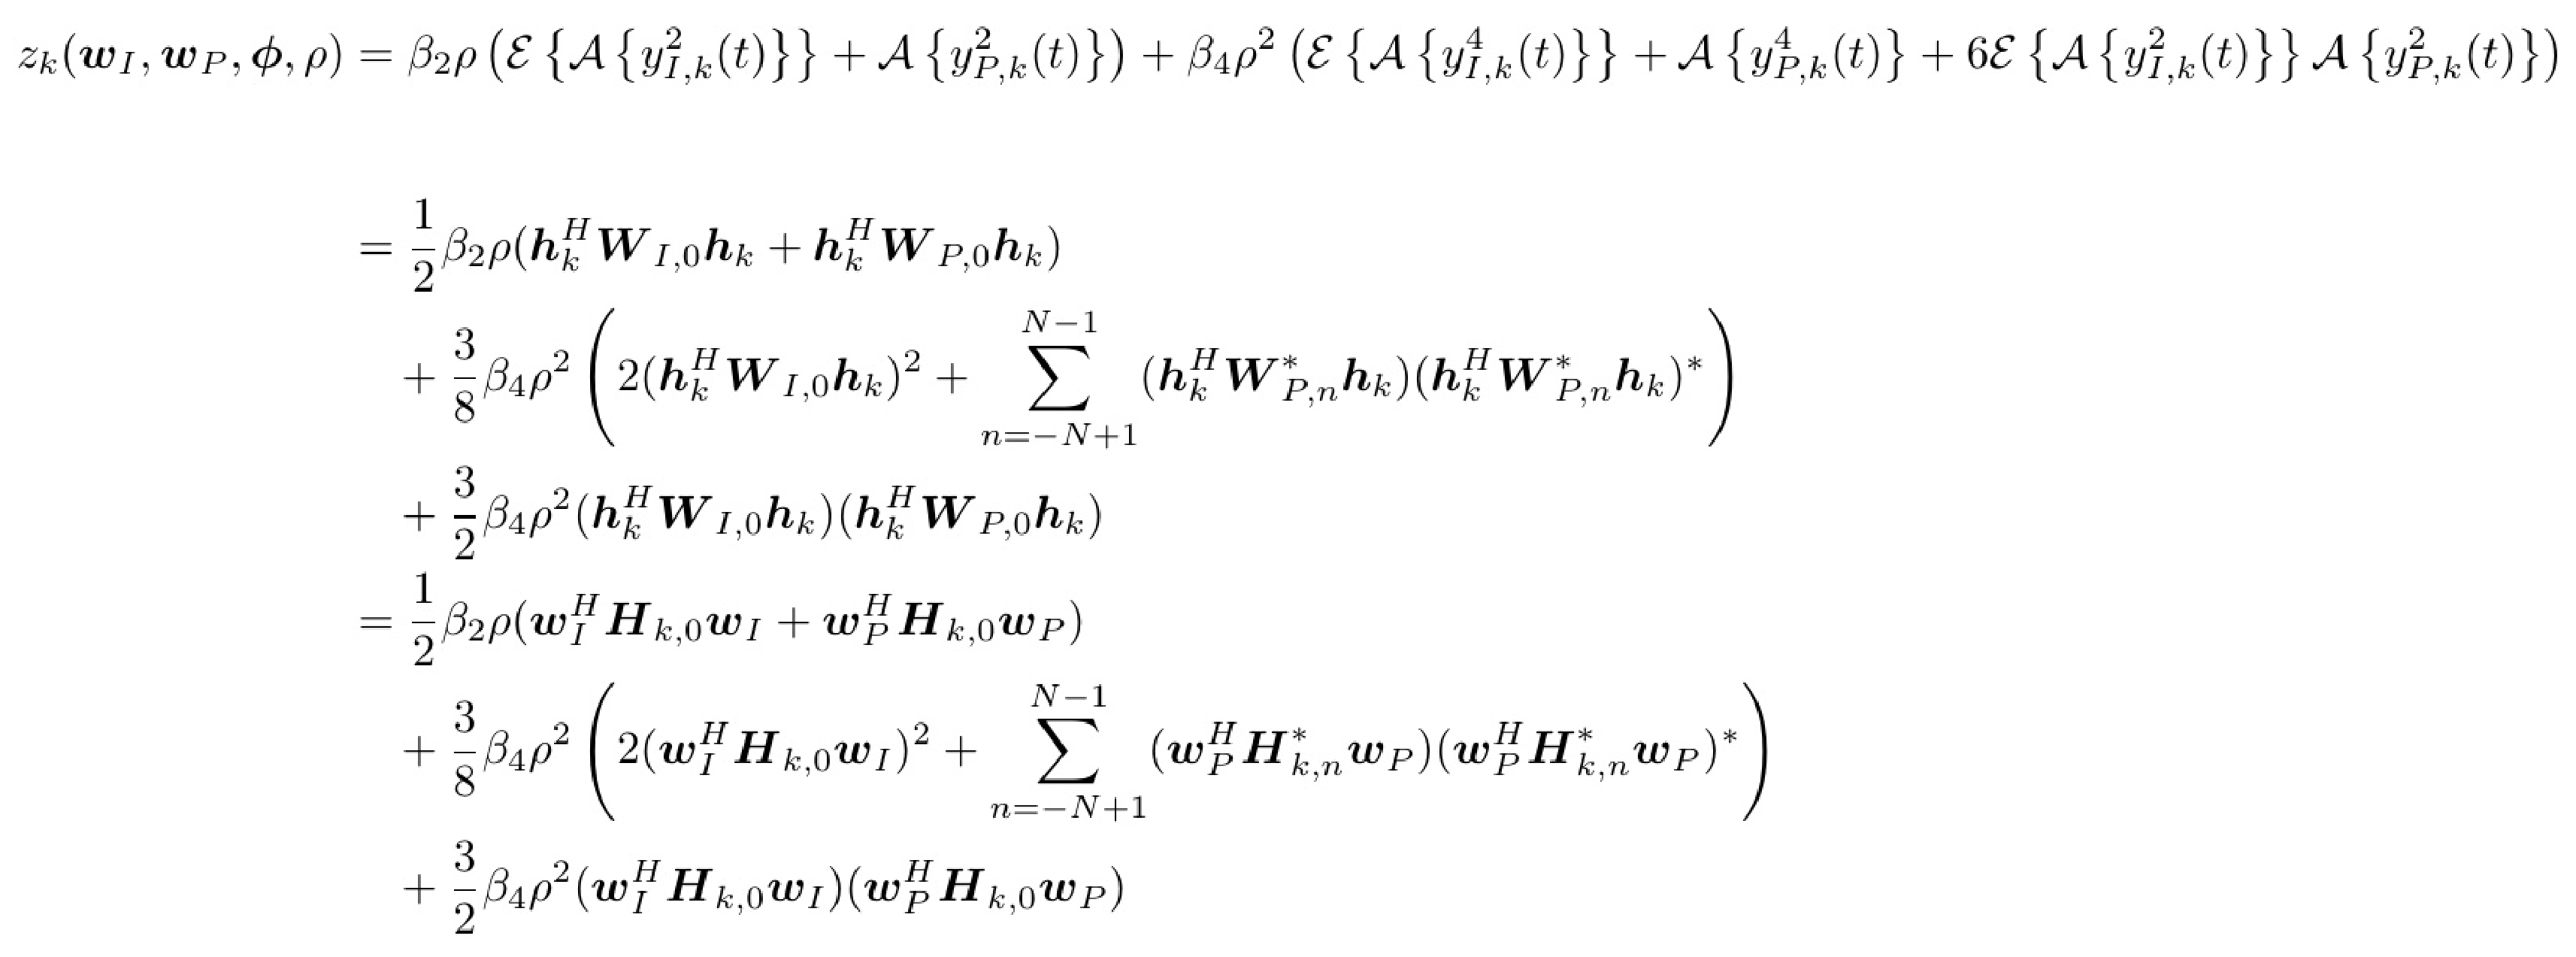
\includegraphics[width=\linewidth]{assets/z.eps}
			\end{figure}
		\end{frame}
	\end{subsection}

	\begin{subsection}{Rate-energy region}
		\begin{frame}{Rate-energy region}
			Define the achievable weighted sum \textbf{R-E region} as
			\begin{equation}
				\begin{split}
					C_{R-I}(P)
					&\triangleq \biggl\{(R,Z):R\le\sum_{k=1}^K{u_{I,k}R_k},Z\le\sum_{k=1}^K u_{P,k}z_k,\\
					&\quad \frac{1}{2}({\boldsymbol{w}_I^H}{\boldsymbol{w}_I}+{\boldsymbol{w}_P^H}{\boldsymbol{w}_P}) \le P\biggr\}
				\end{split}
			\end{equation}
			\begin{itemize}
				\item $P$ is the transmit power budget
				\item $u_{I/P,k}$ are the information and power weight of user $k$
			\end{itemize}
		\end{frame}
	\end{subsection}
\end{section}

\begin{section}{Single-user optimization}
	\begin{subsection}{Problem formulation}
		\begin{frame}{Problem formulation}
			We characterize the rate-energy region through a current maximization problem subject to transmit power, rate, and IRS constraints
			\begin{maxi!}
				{\boldsymbol{w}_I,\boldsymbol{w}_P,\boldsymbol{\phi},\rho}{z(\boldsymbol{w}_I,\boldsymbol{w}_P,\boldsymbol{\phi},\rho)}{\label{op:su}}{\label{eq:su_target}}
				\addConstraint{\frac{1}{2}({\boldsymbol{w}_I^H}{\boldsymbol{w}_I}+{\boldsymbol{w}_P^H}{\boldsymbol{w}_P})\le{P}}
				\addConstraint{\sum_{n}{\log_2\left(1+\frac{(1-\rho)\lvert(h_{D,n}+\boldsymbol{v}_n^H\boldsymbol{\phi})w_{I,n}\rvert^2}{\sigma_n^2}\right)} \ge \bar{R}}\label{eq:su_rate_constraint}
				\addConstraint{\lvert{\phi_l}\rvert=1, \quad l=1,\dots,L}
				\addConstraint{0 \le \rho \le 1}
			\end{maxi!}
			\vspace{1em}
			$\boldsymbol{w}_{I/P},\boldsymbol{\phi},\rho$ are coupled in \ref{eq:su_target}, \ref{eq:su_rate_constraint}, consider \textbf{alternating optimization} (AO).
		\end{frame}
	\end{subsection}

	\begin{subsection}{IRS phase shift}
		\begin{frame}{Frequency-selective IRS}
			The ideal \textbf{Frequency-Selective} (FS) IRS provides:
			\begin{itemize}
				\item subband-dependent reflection coefficients ($\boldsymbol{\phi}_n$ replaces $\boldsymbol{\phi}$)
				\item total DoF $NL$
			\end{itemize}
			\vspace{1em}
			Note that $\lvert{(h_{D,n}+\boldsymbol{v}_n^H\boldsymbol{\phi}_n)w_{I,n}}\rvert \le \lvert{h_{D,n}w_{I,n}}\rvert+\lvert{\boldsymbol{v}_n^H\boldsymbol{\phi}_n w_{I,n}}\rvert$ and the equality holds when the direct and IRS-aided links are aligned. Therefore, we simply select the phase shift of element $l$ at subband $n$ as
			\begin{equation}
				\theta_{n,l}^\star = \angle{h}_{D,n} - \angle{h_{R,n,l}}-\angle{h_{I,n,l}}
			\end{equation}
			That is to say, the optimal phase shift for FS-IRS is obtained in closed form in the single-user scenario, which ensures the direct, extra and composite channels have the same phase.
		\end{frame}

		\begin{frame}{Frequency-flat IRS (1)}
			\textbf{Frequency-Flat} (FF) IRS reflects all subbands equally with a DoF of $L$.
			\begin{block}{Semi-Definite Relaxation (SDR): rate constraint}
				To simplify rate constraint \ref{eq:su_rate_constraint}, we observe that
				\begin{equation}
					\begin{split}
						\lvert{h_{D,n}+\boldsymbol{v}_n^H\boldsymbol{\phi}}\rvert^2
						&=\lvert{h_{D,n}}\rvert^2+h_{D,n}^*\boldsymbol{v}_n^H\boldsymbol{\phi}+\boldsymbol{\phi}^H\boldsymbol{v}_n{h_{D,n}}+\boldsymbol{\phi}^H\boldsymbol{v}\boldsymbol{v}^H\boldsymbol{\phi}\\
						&=\bar{\boldsymbol{\phi}}^H\boldsymbol{R}_n\bar{\boldsymbol{\phi}}=\mathrm{Tr}(\boldsymbol{R}_n\bar{\boldsymbol{\phi}}\bar{\boldsymbol{\phi}}^H)=\mathrm{Tr}(\boldsymbol{R}_n\boldsymbol{\Phi})
					\end{split}
				\end{equation}
				where $t$ is an auxiliary variable with unit modulus and
				\begin{equation}\label{eq:R_n,phi}
					\boldsymbol{R}_n=
					\begin{bmatrix}
						\boldsymbol{v}_n\boldsymbol{v}_n^H & \boldsymbol{v}_n{h_{D,n}} \\
						h_{D,n}^*{\boldsymbol{v}_n^H}      & h_{D,n}^*{h_{D,n}}
					\end{bmatrix},
					\quad \bar{\boldsymbol{\phi}}=\
					\begin{bmatrix}
						\boldsymbol{\phi} \\
						t
					\end{bmatrix},
					\quad \boldsymbol{\Phi}=\bar{\boldsymbol{\phi}}\bar{\boldsymbol{\phi}}^H
				\end{equation}
			\end{block}
		\end{frame}

		\begin{frame}{Frequency-flat IRS (2)}
			We optimize $\boldsymbol{\Phi}$ with given waveform $\boldsymbol{w}_{I/P}$ and splitting ratio $\rho$.
			\begin{block}{SDR: current expression}
				Define $\boldsymbol{M}=[\boldsymbol{V}^H,\boldsymbol{h}_D]^H$ such that $\boldsymbol{h}\boldsymbol{h}^H=\boldsymbol{M}^H\boldsymbol{\Phi}\boldsymbol{M}$. Introduce auxiliary variables
				\begin{equation}\label{eq:t}
					\begin{split}
						t_{I/P,n}
						&=\boldsymbol{h}^H\boldsymbol{W}_{I/P,n}^*\boldsymbol{h}=\mathrm{Tr}(\boldsymbol{h}\boldsymbol{h}^H\boldsymbol{W}_{I/P,n}^*)=\mathrm{Tr}(\boldsymbol{M}^H\boldsymbol{\Phi}\boldsymbol{M}\boldsymbol{W}_{I/P,n}^*)\\
						&=\mathrm{Tr}(\boldsymbol{M}\boldsymbol{W}_{I/P,n}^*\boldsymbol{M}^H\boldsymbol{\Phi})=\mathrm{Tr}(\boldsymbol{C}_{I/P,n}\boldsymbol{\Phi})
					\end{split}
				\end{equation}
				Therefore, the current expression rewrites as
				\begin{equation}\label{eq:z_irs}
					z(\boldsymbol{\Phi})=\frac{1}{2}{\beta_2}{\rho}(t_{I,0}+t_{P,0})+\frac{3}{8}{\beta_4}{\rho^2} \left(2t_{I,0}^2 + \sum_{n=-N+1}^{N-1}{t_{P,n}t_{P,n}^*}\right)+\frac{3}{2}{\beta_4}{\rho^2}t_{I,0}t_{P,0}
				\end{equation}
			\end{block}
		\end{frame}

		\begin{frame}{Frequency-flat IRS (3)}
			We use first-order Taylor expansion to approximate the second-order terms in \ref{eq:z_irs}. Based on the variables optimized at iteration $i - 1$, the local approximation at iteration $i$ gives
			\begin{align}
				(t_{I,0}^{(i)})^2
				& \ge 2 t_{I,0}^{(i)}t_{I,0}^{(i-1)} - (t_{I,0}^{(i-1)})^2\label{eq:t_{I,0}_square}\\
				t_{P,n}^{(i)} (t_{P,n}^{(i)})^*
				& \ge 2 \Re\left\{t_{P,n}^{(i)} (t_{P,n}^{(i-1)})^*\right\} - t_{P,n}^{(i-1)} (t_{P,n}^{(i-1)})^*\\
				t_{I,0}^{(i)} t_{P,0}^{(i)}
				& = \frac{1}{4}(t_{I,0}^{(i)} + t_{P,0}^{(i)})^2 - \frac{1}{4}(t_{I,0}^{(i)} - t_{P,0}^{(i)})^2\nonumber\\
				& \ge \frac{1}{2}(t_{I,0}^{(i)} + t_{P,0}^{(i)})(t_{I,0}^{(i-1)} + t_{P,0}^{(i-1)})\nonumber\\
				& \quad - \frac{1}{4}(t_{I,0}^{(i-1)} + t_{P,0}^{(i-1)})^2 - \frac{1}{4}(t_{I,0}^{(i)} - t_{P,0}^{(i)})^2\label{eq:t_{I/P,0}}
			\end{align}
		\end{frame}

		\begin{frame}{Frequency-flat IRS (4)}
			Hence, problem \ref{op:su} is transformed to
			\begin{maxi!}
				{\boldsymbol{\boldsymbol{\Phi}}}{\tilde{z}(\boldsymbol{\Phi})}{\label{op:su_irs}}{\label{eq:su_irs_target}}
				\addConstraint{\sum_{n}{\log_2\left(1+\frac{(1-\rho)\lvert{w}_{I,n}\rvert^2\mathrm{Tr}(\boldsymbol{R}_n\boldsymbol{\Phi})}{\sigma_n^2}\right)} \ge \bar{R}}
				\addConstraint{\boldsymbol{\Phi}_{l,l}=1, \quad l=1,\dots,L+1}
				\addConstraint{\boldsymbol{\Phi}\succeq{0}}
				\addConstraint{\mathrm{rank}(\boldsymbol{\Phi})=1\label{co:irs_rank}}
			\end{maxi!}
		\end{frame}
	\end{subsection}

	\begin{subsection}{Waveform}
		\begin{frame}{Waveform (1)}
			We optimize $\boldsymbol{w}_{I/P}$ with given IRS $\boldsymbol{\phi}$ and splitting ratio $\rho$.
			\begin{block}{SDR: current expression}
				Introduce auxiliary variables
				\begin{equation}\label{eq:t'}
					t_{I/P,n}' = \boldsymbol{w}_{I/P}^H \boldsymbol{H}_n^* \boldsymbol{w}_{I/P} = \mathrm{Tr}(\boldsymbol{H}_n^*\boldsymbol{W}_{I/P})
				\end{equation}
				Therefore, the current expression rewrites as
				\begin{equation}\label{eq:z_waveform}
					z(\boldsymbol{W}_{I/P})=\frac{1}{2} \beta_2 \rho (t'_{I,0}+t'_{P,0})+\frac{3}{8} \beta_4 \rho^2 \left(2(t'_{I,0})^2 + \sum_{n=-N+1}^{N-1}{t'_{P,n}(t'_{P,n})^*}\right)+\frac{3}{2} \beta_4 \rho^2 t'_{I,0}t'_{P,0}
				\end{equation}
				Since \ref{eq:z_waveform} and \ref{eq:z_irs} are in the same form, we use same Taylor approximation.
			\end{block}
		\end{frame}

		\begin{frame}{Waveform (2)}
			Hence, problem \ref{op:su} is transformed to
			\begin{maxi!}
				{\boldsymbol{W}_{I/P}}{\tilde{z}(\boldsymbol{W}_I,\boldsymbol{W}_P)}{\label{op:su_waveform}}{\label{eq:su_waveform_target}}
				\addConstraint{\sum_{n}{\log_2\left(1+\frac{(1-\rho)W_{I,n,n}\lvert h_n \rvert^2}{\sigma_n^2}\right)} \ge \bar{R}\label{eq:su_waveform_constraint}}
				\addConstraint{\frac{1}{2}\left(\mathrm{Tr}(\boldsymbol{W}_I)+\mathrm{Tr}(\boldsymbol{W}_P)\right) \le P}
				\addConstraint{\boldsymbol{W}_{I/P} \succeq 0}
				\addConstraint{\mathrm{rank}(\boldsymbol{W}_{I/P})=1\label{co:waveform_rank}}
			\end{maxi!}
		\end{frame}
	\end{subsection}

	\begin{subsection}{Splitting ratio}
		\begin{frame}{Splitting ratio}
			We optimize $\rho$ with given IRS $\boldsymbol{\phi}$ and waveform $\boldsymbol{w}_{I/P}$.
			\begin{maxi!}
				{\rho}{z(\rho)}{\label{op:su_ratio}}{\label{eq:su_ratio_target}}
				\addConstraint{\sum_{n}{\log_2\left(1+\frac{(1-\rho)\lvert h_n w_n \rvert^2}{\sigma_n^2}\right)} \ge \bar{R}\label{eq:su_ratio_constraint}}
				\addConstraint{0 \le \rho \le 1}
			\end{maxi!}
			Since $z(\rho)$ is a quadratic function that monotonically increases over $\rho \in [0, 1]$, we replace $z(\rho)$ with affine $\rho$ and solve problem \ref{op:su_ratio}.
		\end{frame}
	\end{subsection}
\end{section}

\bibliographystyle{IEEEtran}
\bibliography{library.bib}
\end{document}
